%%%%%%%%%%%%%%%%%%%%%%%%%%%%%%%%%%%%%%%%%%%%%%%%%%%%%%%%%%%%%%%%%%%%%%
% Overleaf (WriteLaTeX) Example: Molecular Chemistry Presentation
%
% Source: http://www.overleaf.com
%
% In these slides we show how Overleaf can be used with standard 
% chemistry packages to easily create professional presentations.
% 
% Feel free to distribute this example, but please keep the referral
% to overleaf.com
% 
%%%%%%%%%%%%%%%%%%%%%%%%%%%%%%%%%%%%%%%%%%%%%%%%%%%%%%%%%%%%%%%%%%%%%%
% How to use Overleaf: 
%
% You edit the source code here on the left, and the preview on the
% right shows you the result within a few seconds.
%
% Bookmark this page and share the URL with your co-authors. They can
% edit at the same time!
%
% You can upload figures, bibliographies, custom classes and
% styles using the files menu.
%
% If you're new to LaTeX, the wikibook is a great place to start:
% http://en.wikibooks.org/wiki/LaTeX
%
%%%%%%%%%%%%%%%%%%%%%%%%%%%%%%%%%%%%%%%%%%%%%%%%%%%%%%%%%%%%%%%%%%%%%%

\documentclass[xcolor=dvipsnames]{beamer}

\usetheme{Madrid}
\useoutertheme{split} % Alternatively: miniframes, infolines, split
\useinnertheme{circles}

%%%%%%%%%%
% Giorgio Morandi #colors_1
\definecolor{color0}{HTML}{372639}
\definecolor{color1}{HTML}{C2A4C0}
\definecolor{color2}{HTML}{816288}
\definecolor{color3}{HTML}{C6926C}
\definecolor{color4}{HTML}{D5BEA9}
\definecolor{color5}{HTML}{DBCAD3}
%%%%%%%%%%

%%%%%%%%%%
\setbeamercolor{normal text}{bg = color5!25, fg = color0}
%\setbeamercolor{alerted text}{bg = color5, fg = color1}
%\setbeamercolor{example text}{bg = color5, fg = color1!50!color0}

\setbeamercolor{palette primary}{bg = color3, fg = color5!50}
%\setbeamercolor{palette secondary}{bg = color1, fg = color5}
%\setbeamercolor{palette tertiary}{bg = color4, fg = color5}

\setbeamercolor{palette quaternary}{bg = color2!50, fg = color0!75}

\setbeamercolor{structure}{bg = color5!50, fg = color4} % itemize, enumerate, etc

\setbeamercolor{section in toc}{bg = color5!50, fg = color1} % TOC sections

% Override palette coloring with secondary
\setbeamercolor{subsection in head/foot}{bg = color3!50, fg = color2}
% For more themes, color themes and font themes, see:
% http://deic.uab.es/~iblanes/beamer_gallery/index_by_theme.html
%%%%%%%%%%

%%%%%%%%%%
\mode<presentation>
{
  \usetheme{Madrid}       % or try default, Darmstadt, Warsaw, ...
  \usecolortheme{default} % or try albatross, beaver, crane, ...
  \usefonttheme{serif}    % or try default, structurebold, ...
  \setbeamertemplate{navigation symbols}{}
  \setbeamertemplate{caption}[numbered]
} 

\usepackage[english, french]{babel}
\usepackage[utf8x]{inputenc}
\usepackage{chemfig}
\usepackage[version = 3]{mhchem}

% On Overleaf, these lines give you sharper preview images.
% You might want to `comment them out before you export, though.
\usepackage{pgfpages}
\pgfpagesuselayout{resize to}[%
  physical paper width = 8in, physical paper height = 6in]
  
% Here's where the presentation starts, with the info for the title slide
\title[SYSTÈMES INTELLIGENTS]{\textsc{SYSTÈMES INTELLIGENTS \\\normalsize{POUR LA TRANSMISSION DES \\HUMANITÉS NUMÉRIQUES \\ET POUR LA RECHERCHE EN SANTÉ}}}
\institute{\large{\texttt{ELLIADD}}}
\author{Directeur de thèse (HDR) : Thibaud HULIN
\\Présentateur : Hao ZHANG}

\usepackage{datetime}
\newdate{date}{25}{6}{2021}
\date{\displaydate{date}}
%\date{11 novembre 2018}

\logo{\includegraphics[height = 10mm]{images/logo ELLIADD.png}}

\setbeamersize{text margin left = 0.25in, text margin right = 0.25in}

\usepackage{ragged2e}
\renewcommand{\raggedright}{\leftskip=0pt \rightskip=0pt plus 0.25in}

\begin{document}

\begin{frame}
	\titlepage
\end{frame}

\section{À propos de moi}

\begin{frame}
	\frametitle{Sommaire}
	\tableofcontents[currentsection]
\end{frame}

\begin{frame}[fragile]
	\frametitle{À propos de moi}
		\begin{block}{Formation}
			\begin{itemize}
				\item[$\bullet$]Étudiant de Mastère Spécialisé Smart System \& IoT (Internet of Things) de CY Tech (ex.: EISTI)
				\item[$\bullet$]Ingénieur Diplômé de l’ESLIV en IBO(Informatique, Big Data et Object Connecté en option de data science
				\item[$\bullet$]šFormation 5 ans de médecine pour la licence. Participé à un programme d’échange franco-chinois sur la médecine d’urgences.
			\end{itemize}
		\end{block}
\end{frame}

\begin{frame}[fragile]
\frametitle{À propos de moi}
\begin{block}{Expérience}
	\begin{itemize}
		\item[$\bullet$]Maîtriser bien de certains langages de programmation et manipuler certains types de bases de données
		\item[$\bullet$]Connaître bien le domaine de Data Science, Machine Learning, TAL et IoT et participer certains projets d’IA (traitement d’image, traitement de langage, etc.)
		\item[$\bullet$]Plus d’un an d’expérience dans une entreprise pharmaceutique en étudiant de nouveaux médicaments et leur résultat d’essai clinique.
	\end{itemize}
\end{block}
\end{frame}

\section{Humanités Numériques (HN)}

\begin{frame}
\frametitle{Sommaire}
\tableofcontents[currentsection]
\end{frame}

\begin{frame}{Humanités Numériques (HN)}
\begin{columns}
	\column{0.6\textwidth}
		\begin{itemize}
		\item[$\bullet$] Les Humanités Numériques (HN) forment un socle de partage, d'étude et de formation à des concepts ou à des compétences de haut niveau (dont dépendent les autres compétences), pour apprendre avec les technologies numériques.
		
		\item[$\bullet$] Avec les HN, l’IA facilite la reconnaissance des textes manuscrits dans les archives, la recherche d’information et la représentation des données via des graphes.
	\end{itemize}	
	\column{0.4\textwidth}
	\begin{figure}[ht]
		\begin{center}
			\includegraphics[width=\textwidth]{./images/Humanites_Numeriques.JPG}
		\end{center}
	\end{figure}
\end{columns}
\end{frame}

\section{À propos de projet}

\begin{frame}
\frametitle{Sommaire}
\tableofcontents[currentsection]
\end{frame}

\subsection{Synthèse de projet}
% Page_5
\begin{frame}[fragile]
\frametitle{Synthèse de projet}
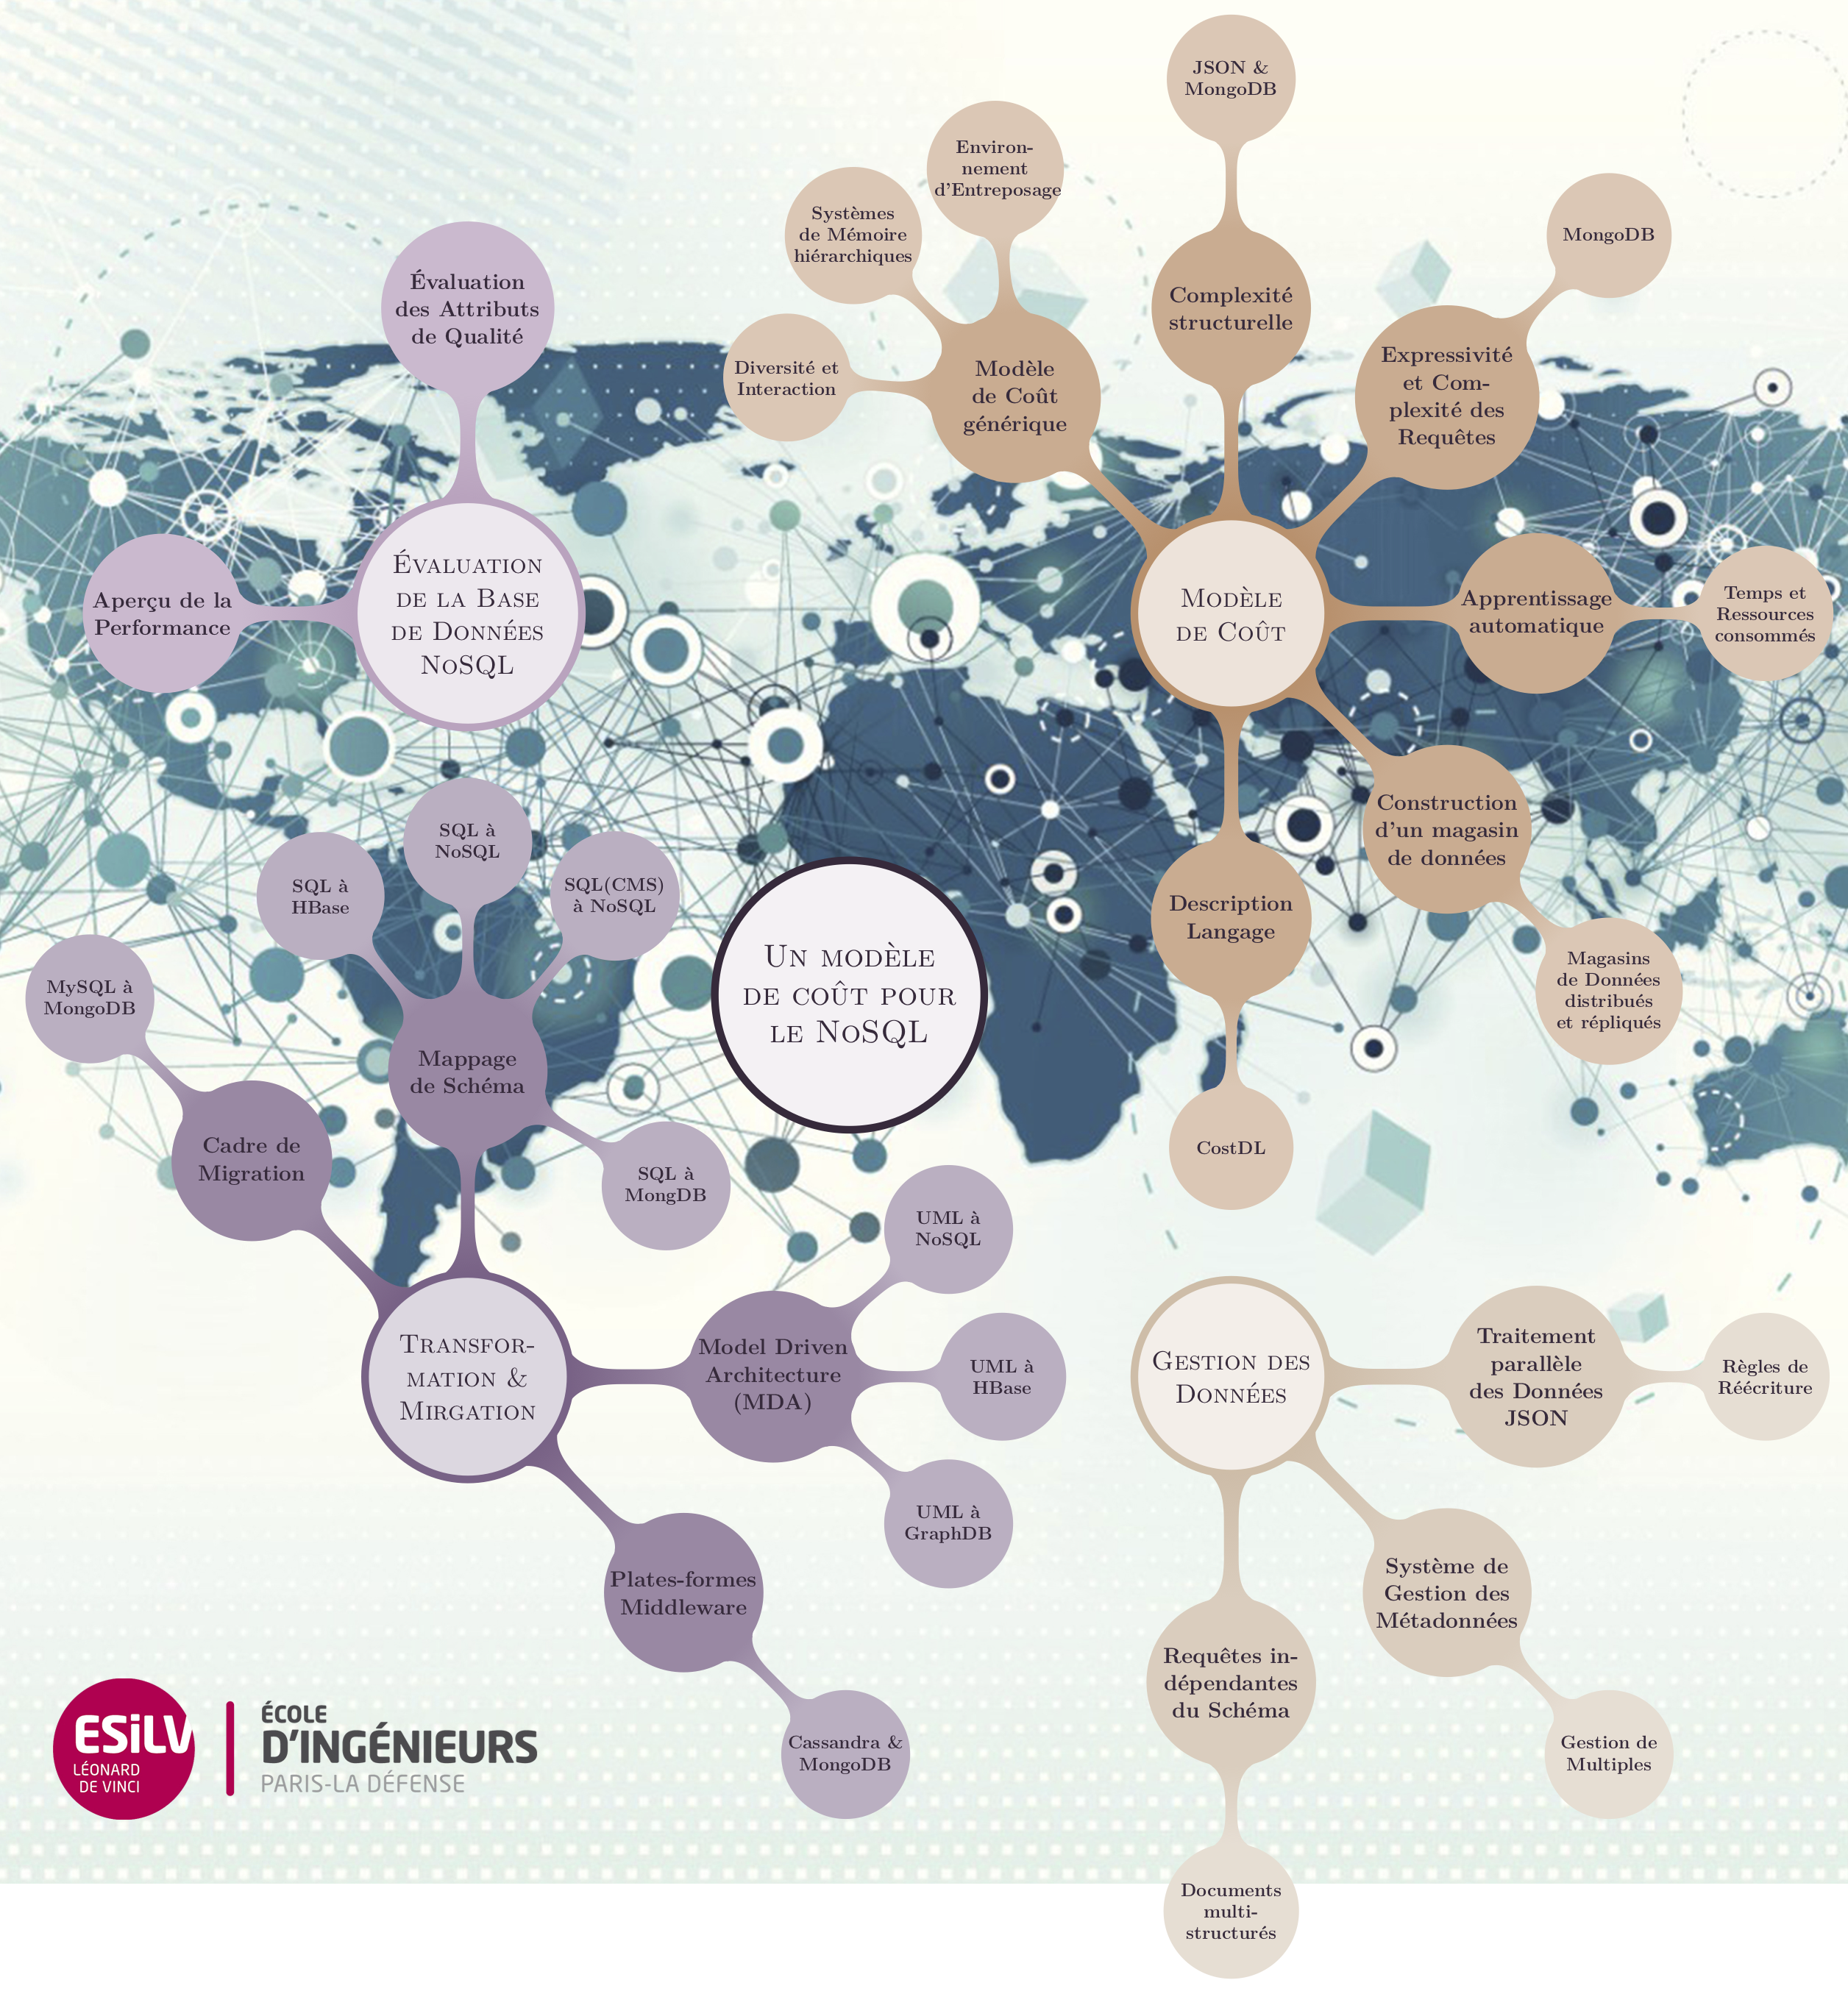
\includegraphics[height = 7cm]{images/mindmap.png}
\end{frame}

% Page_6
%\subsection{Problématique \& Enjeux}
%\begin{frame}[fragile]
%	\frametitle{Problématique \& Enjeux}
%	\begin{columns}
%	\column{0.45\textwidth}
%	\begin{block}{Problématique}
%	\end{block}
%	\column{0.45\textwidth}
%	\begin{block}{Enjeux}
%	\end{block}
%\end{columns}
%\end{frame}

% Page_7
\subsection{Objectifs de la recherche en IA
}
\begin{frame}[fragile]
\frametitle{Objectifs de la recherche en IA
}
\begin{columns}
	\column{0.475\textwidth}
	\begin{block}{Données}
		\begin{itemize}
			\item[$\bullet$] les scénarios de cours produits par les enseignants
			\item[$\bullet$] les fonds d’archives numérisés, à valoriser en pédagogie, et pour les chercheurs (notamment du pôle thématique LLC)
		\end{itemize}	
	\end{block}
	\column{0.475\textwidth}
	\begin{block}{IA}
		\begin{itemize}
		\item[$\bullet$] permet de suggérer des ressources en lien pour les enseignants
		\item[$\bullet$] permet de visualiser les données pour les chercheurs
		\end{itemize}
	\end{block}
\end{columns}
\end{frame}

\subsection{Démarche globale}
% Page_9
\begin{frame}[fragile]
\frametitle{Démarche globale
}
\begin{block}{Démarche globale 1 / 2}
	\begin{itemize}
		\item[$\bullet$] Cartographier le champ grâce à la mobilisation d’experts du domaine.
		\item[$\bullet$] Collecter les données d’expérience pédagogiques sur une plateforme dédiée.
		\item[$\bullet$] Concevoir services en comparant des cas d'utilisation en santé et en humanités.
	\end{itemize}
\end{block}
\end{frame}

\begin{frame}{Concevoir les services en utilisant web sémantique}
\begin{columns}
	\column{1.05\textwidth}
	\begin{itemize}
	\item[$\bullet$] World Wide Web Consortium (W3C) est une institution mondiale d’Internet public, qui est reconnu comme le leader dans le web sémantique et en sciences cognitives. La co-directrice de thèse, D. McGuiness en fait partie et y contribue. 
	\end{itemize}
\end{columns}
	\begin{columns}
	\column{0.6\textwidth}
	\begin{itemize}
		\item[$\bullet$] Le Web sémantique est une extension du Web standardisée par le W3C. Ces standards encouragent l'utilisation de formats de données et de protocoles d'échange normés sur le Web, en s'appuyant sur le modèle Resource Description Framework (RDF) qui est la technologie centrale du Web sémantique. 
	\end{itemize}
	\column{0.425\textwidth}
	\begin{figure}[ht]
		\begin{center}
			\includegraphics[width=\textwidth]{./images/Semantic_Web.png}
		\end{center}
	\end{figure}
\end{columns}
\end{frame}

\begin{frame}[fragile]
\frametitle{Démarche globale}
\begin{block}{Démarche globale 2 / 2}
	\begin{itemize}
		\item[$\bullet$] Développer des services intelligents pour la recherche d'information, la visualisation et l’analyse des données.
		\item[$\bullet$] Évaluer les usages (analyse des traces, mouvements oculaires, enquêtes...).
		\item[$\bullet$] Observer les pratiques d'enseignement et la communication sur le projet.
	\end{itemize}
\end{block}
\end{frame}

\begin{frame}[fragile]
\frametitle{Web sémantique et intelligence artificielle}
\begin{columns}
	\column{0.475\textwidth}
	\begin{block}{Rôle de Web sémantique}
		\begin{itemize}
			\item[$\bullet$] šmodéliser le domaine d'un discours
			\item[$\bullet$] šidentifier les éléments (terminologie), les relations, notamment entre classes et individus
			\item[$\bullet$] šconstruire une ontologie (base de connaissance)
		\end{itemize}
	\end{block}
	\column{0.475\textwidth}
	\begin{block}{Rôle de Web sémantique}
		\begin{itemize}
			\item[$\bullet$] štrouver des régularités
			\item[$\bullet$]suggérer des ressources connexes
			\item[$\bullet$] šconstruire automatiquement une ontologie à partir d'un corpus de textes (via une intelligence artificielle de type connexionnisme)
		\end{itemize}
	\end{block}
\end{columns}
\end{frame}

\begin{frame}[fragile]
\frametitle{Exemple d’ontologie}
\begin{block}{Prototype d‘ontologie}
	\includegraphics[height = 5cm]{images/Ontologie_1.png}
\end{block}
\end{frame}

\begin{frame}[fragile]
\frametitle{Exemple d’ontologie}
\begin{block}{Ontologie de projet de recherche}
		\includegraphics[height = 5cm]{images/Ontologie_2.png}
\end{block}
\end{frame}



\section{Conclusion}
% Page_8
\begin{frame}
\frametitle{Sommaire}
\tableofcontents[currentsection]
\end{frame}


\subsection{Conclusion}
% Page_9
\begin{frame}[fragile]
	\frametitle{Conclusion}
\end{frame}

\end{document}